\chapter{Introduction}
\label{chap:introduction}

% This is the introduction where you should introduce your work. In general the thing to aim for here is to describe a little bit of the context for your work -- why did you do it (motivation), what was the hoped-for outcome (aims) -- as well as trying to give a brief overview of what you actually did.
% It's often useful to bring forward some ``highlights'' into this chapter (e.g.\ some particularly compelling results, or a particularly
% interesting finding).
% It's also traditional to give an outline of the rest of the document, although without care this can appear formulaic and tedious. Your call.




%%% "describe a little bit of the context for your work"

%% Context (~abstract sentence one: topic of compilers/MLIR)
Compilers are a critical component of computing systems, providing an abstraction % for expressivity, performance, and portability (review: first sentence too long)
from high-level programming languages to the underlying machine ISA.
In the 20\textsuperscript{th} century, compilers were typically monolothic and specific to individual languages, resulting in very poor re-usability.
% Early compilers were hand-crafted, resulting in complex and language-specific implementations. % DONE: This needs to be rephrased!!! No early and no hand-crafted, focus on lack of modularity
The LLVM compiler framework \cite{lattnerLLVMCompilationFramework2004} addressed these problems with a novel and language-independent textual \ac{ir} in \ac{ssa} form, which could be analysed and transformed by a sequence of passes.
Recently, \ac{mlir} \cite{lattnerMLIRScalingCompiler2021a}, has furthered these goals by enabling users to cheaply extend compilers with their own abstractions. %, and automatically provides common infrastructure such as parsing and printing logic for them.




%%% "why did you do it (motivation)"

%% Context/Motivation (~abstract sentence one/two/three: extensible compiler frameworks, how this impacts performance, and that MLIR accept it)
Compiler extensibility is critical for handling the heterogeneous hardware and exotic optimisations of modern workloads.
However, this extensibility comes at a cost, presenting an optimisation boundary between the user and framework code. This boundary arises from the dynamic dispatch of these extensions, precluding optimisations such as ahead-of-time code motion.
This is compounded by the dynamic nature of the data structures and algorithms used by the compiler. For example, pattern rewriting in \ac{mlir} operates on a linked list representation of \ac{ssa} values -- a dynamic, pointer-chasing workload.
This further inhibits optimisations, both as a result of dynamism and not being amenable to other transformations such as vectorisation.
These factors motivate challenging the status quo of LLVM and MLIR implementing user-extensible compiler frameworks in static, ahead-of-time compiled languages.






%%% "what was the hoped-for outcome (aims)"

%% Motivation/aim (~abstract sentence four: why not use dynamic languages/xDSL?)
This challenge takes the form of xDSL \cite{fehrXDSLSidekickCompilation2025}, a reimplementation of \ac{mlir}'s core data structures and \ac{ir} definitions in Python, a dynamically typed, interpreted language.
Using Python allows xDSL to take \ac{mlir}'s goal of user extensibility to even further extremes by leveraging its dynamic features such as runtime meta-programming.
In addition to this, xDSL's interpreted nature avoiding \ac{mlir}'s infamously long build times, and its dynamic typing matching the dynamic nature of the user-extensible compiler framework workload.
% xDSL's implementation in Python avoids the long build times of \ac{mlir} as a result of being interpreted. %, and its expressive syntax and minimal boilerplate allows compiler designers to focus on their task as opposed to the underlying language and framework.
% In addition to this, Python's dynamic typing matches the dynamic nature of the user-extensible compiler framework workload.
However, using Python also has drawbacks, most notably in relation to runtime performance.
This work examines the performance of the pattern rewriting component of the xDSL compiler framework, focussing on the impact of dynamism and contrasting against the current state-of-the-art, \ac{mlir}.



%%% "give a brief overview of what you actually did"

%% Pareto curve of performance and dynamism of workload?

\begin{figure}
    \centering
    \begin{tikzpicture}
        \node[anchor=south west,inner sep=0] (image) at (0,0) {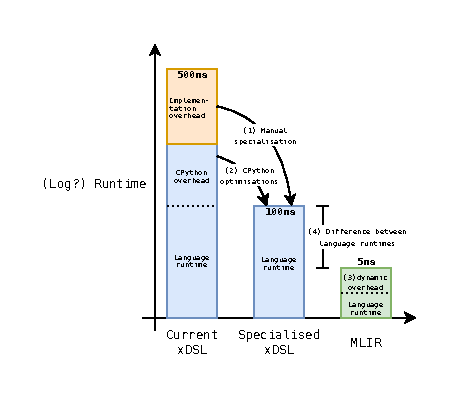
\includegraphics[width=0.6\textwidth]{images/introduction/narrative.drawio.pdf}};
        \node[circledstyle, fill=pairedOneLightBlue] at (4.35,5.05) {1};
        \node[circledstyle, fill=pairedTwoDarkBlue] at (5.55,4.15) {2};
        \node[circledstyle, fill=pairedThreeLightGreen] at (6.95,2.7) {3};
        \node[circledstyle, fill=pairedFourDarkGreen] at (8.75,1.95) {4};
    \end{tikzpicture}
    % 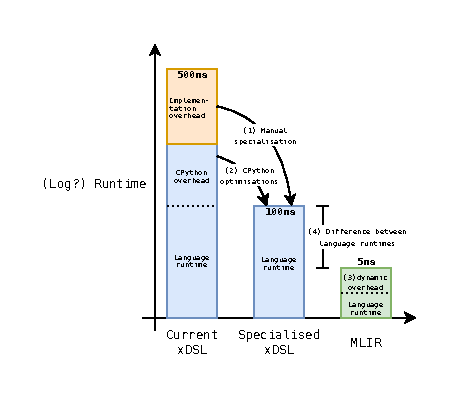
\includegraphics[width=0.6\textwidth]{images/introduction/narrative.drawio.pdf}
    \caption{Closing the gap between xDSL and \ac{mlir} pattern rewriting performance. xDSL's performance can be improved by changes to both its implementation and language runtime. C++ has less of a performance advantage for \ac{mlir} than other workloads due to the costs associated with dynamism.}
    \label{fig:narrative}
\end{figure}

%% Overview (~abstract sentence five, which needs re-writing: what we did part one -- specialisation and CPython stuff)
The performance of a program is constrained both by the details of its implementation and the runtime of its language.
These two properties are deeply interlinked, making them difficult to measure independently.
To disentangle them, we manually optimise and specialise xDSL's implementation of pattern rewriting (\autoref{fig:narrative}, \circledbase{pairedOneLightBlue}{1}), resulting in an $11\times$ performance uplift. % TODO: check alignment with finalised figure when re-measured
We then confirm the performance of the specialisation is constrained only by the language runtime by examination of the dispatched bytecode of micro-benchmarks.
This bytecode examination process revealed a gap in the provision of fine grained performance profilers for Python. To address this gap, we developed ByteSight, native tracing performance profiler for Python bytecode. % TODO: Consider adding "This tool facilitated...?"
Following this, we quantify the impact of recent performance enhancements made to CPython for this specialised implementation (\autoref{fig:narrative}, \circledbase{pairedTwoDarkBlue}{2}). % as an increase of $xy\%$.
This describes the best-case for the performance of pattern rewriting in xDSL, which can then be compared against \ac{mlir}.


%% Overview (~abstract sentence five, which needs re-writing: what we did part two -- custom CPython optimisations)
% Hook
% Argument
% Link


%% Overview (~abstract sentence five, which needs re-writing: what we did part three -- cost of dynamism)
A key difference between the Python and C++ runtimes is their degree of dynamism.
\ac{mlir}'s C++ runtime incurs overhead when dynamically dispatching functions (\autoref{fig:narrative}, \circledbase{pairedThreeLightGreen}{3}), which is worsened by prohibiting ahead-of-time performance optimisations. In contrast, almost every bytecode operation evaluated by the Python interpreter is dynamic, each incurring an overhead.
As such, we expect the difference in performance between language runtimes (\autoref{fig:narrative}, \circledbase{pairedFourDarkGreen}{4}) to be smaller for more dynamic workloads.
To corroborate this, we measure the difference in performance between pattern rewriting workloads using xDSL and \ac{mlir}, and assess the contribution of overheads incurred by dynamism.
This measurement procedure uniquely leverages xDSL's sidekick compilation functionality to ensure the comparability of performance measurements by driving them with the same textual \ac{ir}, even for implementation details internal to each framework.
Finally, we critically evaluate the degree to which this motivates the use of Python for implementing user-extensible compiler frameworks.



%% Contributions (~abstract sentence six: key impact of research)
The contributions of our work are as follows:

\begin{itemize}
    \item An examination of the current %and best-case
    performance of pattern rewriting workloads in the CPython language runtime (\autoref{chap:measuring-compiler-performance}).%(\autoref{chap:measuring-compiler-performance} and \autoref{chap:specialising-optimising-pattern-rewriting} respectively). %, including trade-offs in expressivity and the impact of performance optimisations made to the language runtime.
    \item A tool to examine CPython bytecode dispatch in program runs, facilitating the analysis of costs incurred by dynamism (\autoref{chap:profiling-bytecode}).
    \item A specialisation of the current xDSL implementation for pattern rewriting workloads, demonstrating the best-case performance of CPython for such applications (\autoref{chap:specialising-optimising-pattern-rewriting}).
    \item An exploration of optimisation techniques to shrink the performance gap between dynamic and static languages for pattern rewriting workloads (\autoref{chap:impact-cpython-pattern-rewriting}).
    \item A quantitative comparison of the performance of user-extensible compiler frameworks implemented in static and dynamic languages, focussing on the impact of dynamism (\autoref{chap:dynamism-pattern-rewriting}). % leveraging sidekick compilation for fine-grained analysis of the impact of dynamisms
\end{itemize}
